\section{Results}
\label{sec:results}

\subsection{Explanation Quality Across the Perplexity Spectrum}

\Tabref{tab:main_results} presents explanation quality scores by category. The pattern is strikingly non-monotonic: natural language (4.50) and random tokens (\textbf{5.00}) receive the highest scores, while the three intermediate categories---obfuscated (3.62), human jailbreaks (3.75), and \gcg suffixes (3.75)---score substantially lower.

\begin{table}[t]
    \centering
    \caption{Explanation quality by category. Scores range from 1 (wholly incorrect) to 5 (complete and accurate). Random tokens receive \textbf{perfect} scores despite having high perplexity, revealing a U-shaped pattern rather than monotonic decline. Best scores in \textbf{bold}.}
    \begin{tabular}{@{}lcrcc@{}}
        \toprule
        \textbf{Category} & \textbf{$N$} & \textbf{Median \ppl} & \textbf{Score (mean $\pm$ sd)} & \textbf{Median Score} \\
        \midrule
        Natural language   & 8 &      56.7 & 4.50 {\scriptsize $\pm$ 0.76} & \textbf{5.0} \\
        Obfuscated         & 8 &     334.6 & 3.62 {\scriptsize $\pm$ 0.74} & 3.5 \\
        Human jailbreaks   & 8 &      79.0 & 3.75 {\scriptsize $\pm$ 0.89} & 3.5 \\
        \gcg suffixes      & 8 &   3,493.5 & 3.75 {\scriptsize $\pm$ 1.04} & 4.0 \\
        Random tokens      & 8 &     392.5 & \textbf{5.00} {\scriptsize $\pm$ 0.00} & \textbf{5.0} \\
        \bottomrule
    \end{tabular}
    \label{tab:main_results}
\end{table}

A Kruskal-Wallis test confirms significant differences across categories ($H = 14.96$, $p = 0.005$). \Figref{fig:ushape} visualizes this U-shaped pattern.

\begin{figure}[t]
    \centering
    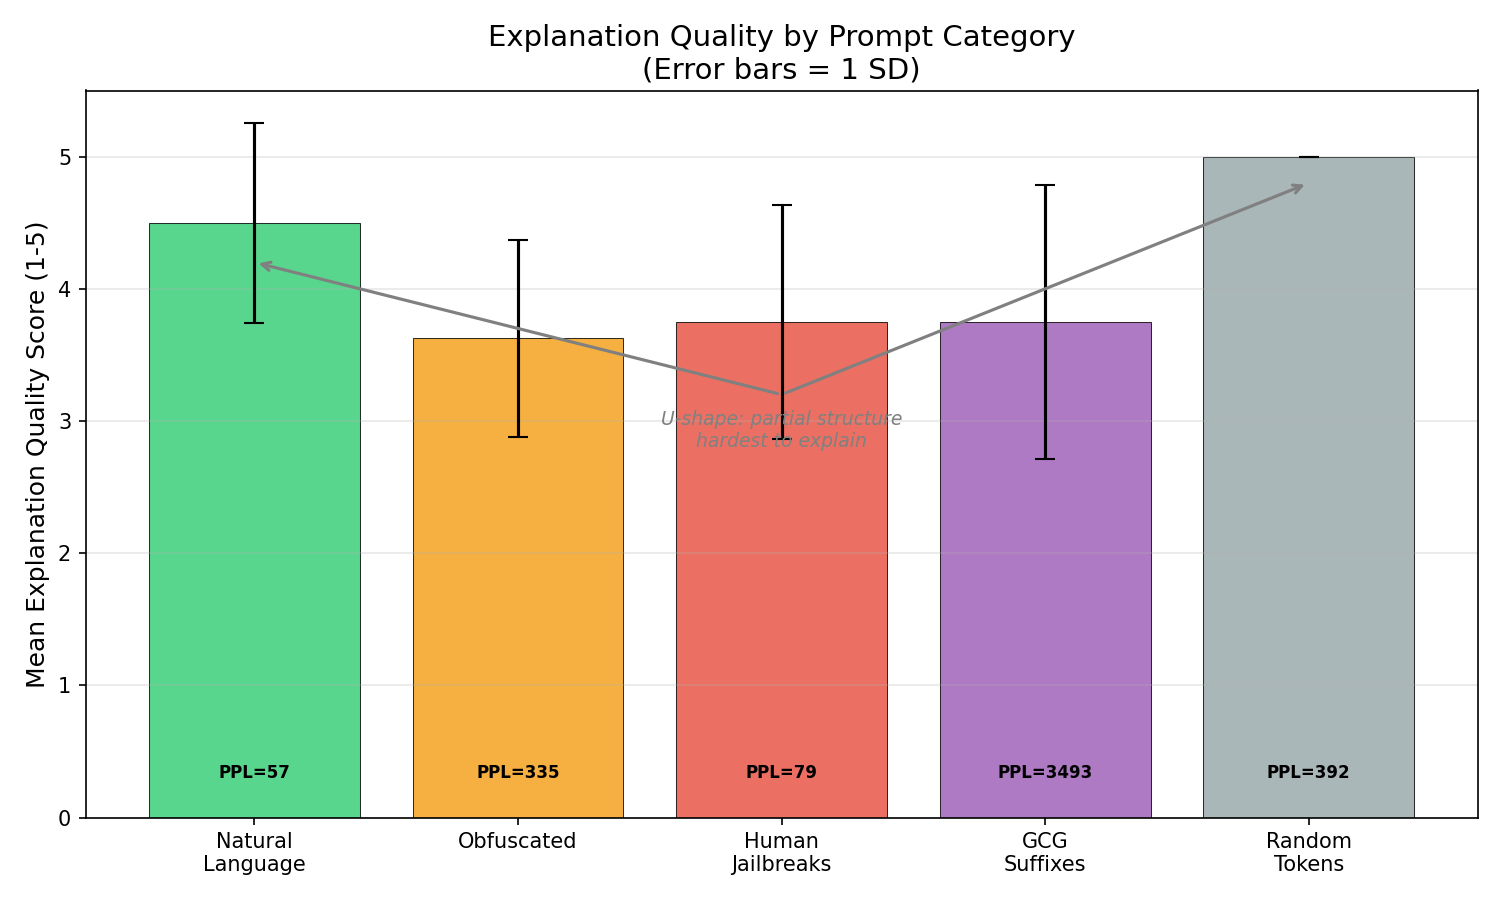
\includegraphics[width=0.85\linewidth]{figures/u_shape_explanation.png}
    \caption{U-shaped explanation quality across five prompt categories ordered by median perplexity. The model explains both natural language (via understanding) and pure random tokens (via \metarecog) well, but struggles with the three intermediate categories that contain partial structure. Error bars show standard deviation.}
    \label{fig:ushape}
\end{figure}

\subsection{Pairwise Comparisons}

\Tabref{tab:pairwise} reports Mann-Whitney $U$ tests for key pairwise comparisons. After Bonferroni correction ($\alpha = 0.005$), random tokens score significantly higher than obfuscated text ($U = 4.0$, $p = 0.001$), human jailbreaks ($U = 8.0$, $p = 0.004$), and \gcg suffixes ($U = 8.0$, $p = 0.004$). The difference between natural language and obfuscated text is suggestive but does not survive correction ($U = 50.5$, $p = 0.045$).

\begin{table}[t]
    \centering
    \caption{Pairwise Mann-Whitney $U$ tests comparing explanation quality between categories. Three comparisons survive Bonferroni correction at $\alpha = 0.005$. All significant results involve random tokens outperforming intermediate categories.}
    \begin{tabular}{@{}llccl@{}}
        \toprule
        \textbf{Comparison} & & $U$ & $p$ & \textbf{Significant?} \\
        \midrule
        Obfuscated    & vs.\ Random     & 4.0  & 0.001 & \textbf{Yes} \\
        Jailbreak     & vs.\ Random     & 8.0  & 0.004 & \textbf{Yes} \\
        \gcg          & vs.\ Random     & 8.0  & 0.004 & \textbf{Yes} \\
        Natural       & vs.\ Obfuscated & 50.5 & 0.045 & No (trend) \\
        \bottomrule
    \end{tabular}
    \label{tab:pairwise}
\end{table}

\subsection{Perplexity Does Not Predict Explanation Quality}

A Spearman correlation between prompt perplexity and explanation score yields $\rho = -0.002$ ($p = 0.992$), indicating no linear relationship. \Figref{fig:scatter} shows the scatter plot: high-perplexity random tokens cluster at score~5, while high-perplexity \gcg suffixes spread across scores~3--5. The relationship is non-monotonic and category-dependent.

\begin{figure}[t]
    \centering
    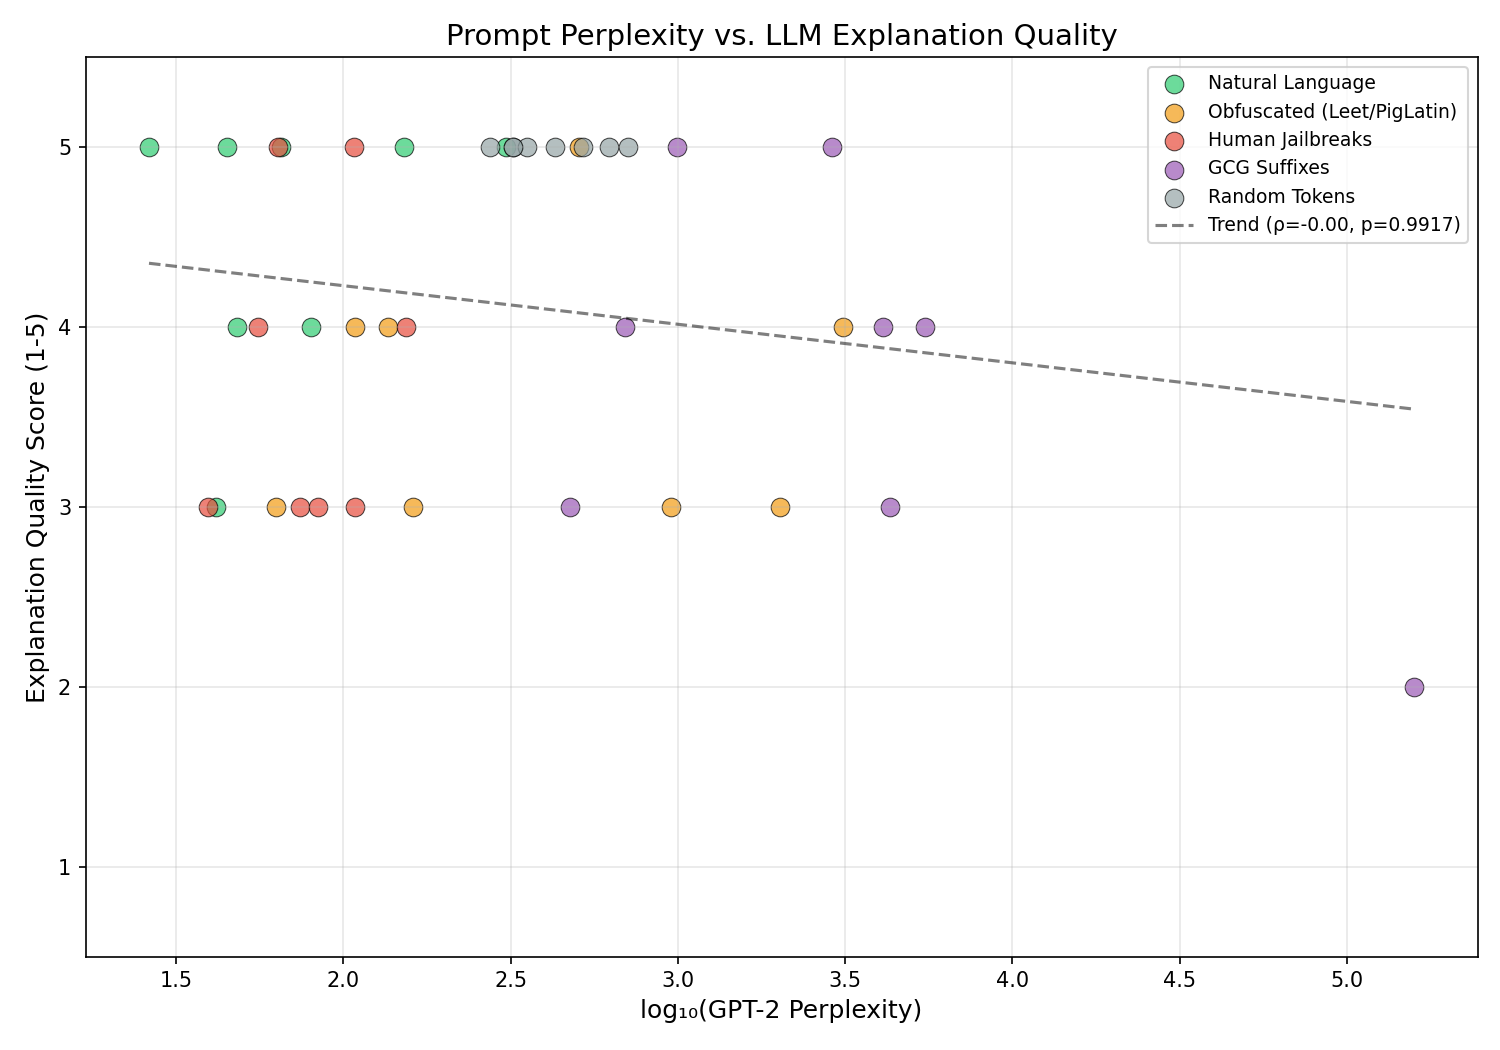
\includegraphics[width=0.85\linewidth]{figures/perplexity_vs_explanation.png}
    \caption{Perplexity vs.\ explanation quality for all 40~prompts, colored by category. There is no linear correlation ($\rho = -0.002$). Random tokens (high perplexity) cluster at score~5 via \metarecog, while \gcg suffixes (very high perplexity) spread across scores~3--5 due to partial confabulation. The dashed line shows the Spearman regression.}
    \label{fig:scatter}
\end{figure}

\subsection{GCG Suffixes Trigger Confabulated Compliance}

Of the 8~\gcg suffixes tested, 5 caused \gptfour to \emph{follow} the prompt rather than flag it as nonsense. Several triggered responses in unexpected languages:
\begin{itemize}[leftmargin=*,itemsep=0pt,topsep=0pt]
    \item The token ``seterusnya'' (Malay for ``next'') triggered a response in Malay about \LaTeX{}.
    \item ``anan diese'' (mixed German/Indonesian) triggered a Spanish response about dice tutorials.
    \item ``Jim komentar hier'' (mixed Dutch/Indonesian) triggered an attempted helpful response about comments.
\end{itemize}

When asked to explain these prompts in Stage~2, \gptfour identified individual trigger tokens correctly (\eg recognizing ``tikzpicture'' and ``tutorial'') but failed to characterize the prompts as adversarial. The model \emph{confabulated} coherent interpretations from fragmentary cues---exactly the behavior adversarial attacks are designed to exploit.

\subsection{Directed Nonsense Search}

Random high-perplexity prompts almost never produce directed model behavior (\tabref{tab:directed}). Only 2 of 30~benign trials (6.7\%) and 1 of 30~jailbreak trials (3.3\%) produced task-relevant outputs. This confirms that directed nonsense requires gradient-based optimization \citep{zou2023universal, cherepanova2024talking}, not random search.

\begin{table}[t]
    \centering
    \caption{Directed nonsense search results. Random token sequences rarely direct models to specific tasks, confirming that gradient-based optimization (\eg \gcg) is essential for crafting effective adversarial prompts.}
    \begin{tabular}{@{}lccl@{}}
        \toprule
        \textbf{Task type} & \textbf{Trials} & \textbf{Successes} & \textbf{Rate} \\
        \midrule
        Benign (poem)       & 30 & 2 & 6.7\% \\
        Jailbreak-adjacent  & 30 & 1 & 3.3\% \\
        \midrule
        Total               & 60 & 3 & 5.0\% \\
        \bottomrule
    \end{tabular}
    \label{tab:directed}
\end{table}
